\hypertarget{instalar_ubuntu_lts}{}

\chapter{Instalar Ubuntu 20.04 LTS}
En este anexo realizaremos la instalación de la distribución Ubuntu 20.04 LTS en su versión para servidores. En este anexo no se va a explicar cómo realizar la creación de una máquina virtual donde se aloja el sistema operativo, ya que existen distintos tipos de virtualizadores.

No se realizará una guía “paso a paso”, sino que se centrará en las partes más importantes de la instalación y en las que más dudas puedan surgir.

\section{Descargar Ubuntu 20.04}
La ISO la obtendremos de la \href{https://ubuntu.com/#download}{web oficial} y seleccionaremos la versión 20.04 LTS de Ubuntu Server. Esta ISO contendrá el sistema base de Ubuntu y nos guiará para realizar la instalación del sistema operativo.

Una vez descargada la ISO tendremos que cargarla en el sistema de virtualización elegido y arrancar la máquina virtual.


\section{Instalar Ubuntu 20.04}
Tras arrancar la máquina virtual nos aparecerá un menú para seleccionar el idioma durante la instalación y le daremos a “Instalar Ubuntu Server”.

\begin{center}
    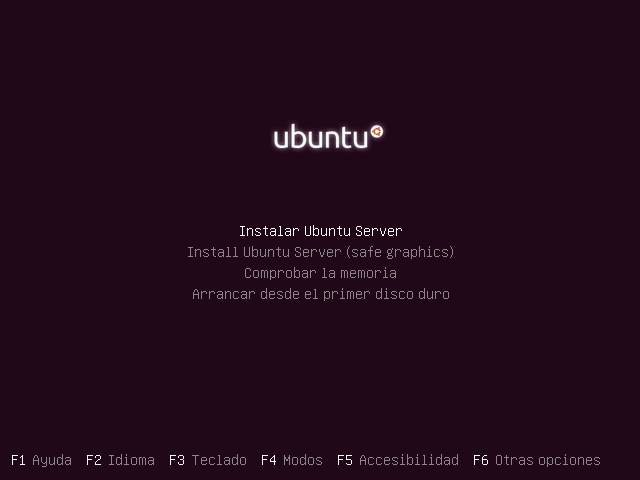
\includegraphics[width=15cm]{ubuntu_1.png}
\end{center}

A partir de aquí comenzará el instalador y los pasos que nos aparecerán serán los siguientes (algunos de estos pasos puede que no estén 100\% traducidos al castellano):

\begin{enumerate}
    \item Elegir el idioma del sistema
    \item Actualización del instalador:
    \begin{itemize}
        \item Si la máquina virtual se puede conectar a internet, comprobará si existe una actualización del propio instalador de Ubuntu.
        \item Podemos darle a “Continuar sin actualizar”
    \end{itemize}
    \item Configuración del idioma del teclado
    \item Configuración de la red
    \item Configuración del proxy de red
    \item Configuración del “mirror” o servidor espejo desde donde descargarse los \hyperlink{paquete_de_software}{paquetes de software} para las actualizaciones posteriores.
    \item Selección del disco duro donde realizar la instalación
    \item Elegir el particionado de disco.
    \item Configuración del perfil. Introduciremos el nombre de usuario, el nombre del servidor y la contraseña del usuario que vamos a crear.
    \item Configuración de SSH Server. Aceptaremos que se instale el servidor SSH durante la instalación. En caso de no seleccionar esta opción, posteriormente podremos realizar la instalación.
    \item “Featured Server Snaps”. En esta pantalla nos permite instalar software muy popular en servidores.
\end{enumerate}


Una vez le demos a continuar, comenzará la instalación en el disco duro. Debido a que durante la instalación tenemos conexión a internet, el propio instalador se descarga las últimas versiones de los paquetes de software desde los repositorios oficiales.


Al terminar la instalación, tendremos que reiniciar la máquina virtual.

\section{Post-instalación}
Tras realizar el reinicio de la máquina virtual nos encontraremos con que el sistema arranca en el sistema recién instalado, y que tendremos que loguearnos introduciendo el usuario y la contraseña utilizadas en la instalación.

\subsection{Actualización del sistema}
Por si acaso, realizaremos la actualización del índice del repositorio, actualizaremos el sistema y en caso necesario realizaremos un nuevo reinicio:

\begin{mycode}{Actualizar Ubuntu}{console}{}
mikeldi@ubuntu:~$ sudo su
[sudo] password for mikeldi:
root@ubuntu:~# apt update
...
root@ubuntu:~# apt upgrade
...
\end{mycode}

Con estos comandos nos aseguramos que el sistema está actualizado a los últimos paquetes que están en el repositorio.

\subsection{Poner IP estática}
Debido a la configuración de red de nuestro servidor, la IP está puesta en modo dinámica, esto quiere decir que nuestro equipo ha cogido la IP por configuración de DHCP de nuestra red. Debido a que un servidor debe de tener IP estática, tenemos que realizar la modificación adecuada para ponerle la IP estática que mejor nos convenga. Para ello editaremos el fichero de configuración situado en la siguiente ruta: \configfile{ /etc/netplan/00-installer-config.yaml }

Lo modificaremos para que sea parecido a (siempre teniendo en cuenta la IP y gateway de nuestra red):


\begin{mycode}{Configurando IP estática en Ubuntu}{yaml}{}
network:
  ethernets:
    enp1s0:
      dhcp4: no
      addresses:
      - 192.168.200.10/24
      gateway4: 192.168.200.1
      nameservers:
        addresses: [8.8.8.8]
  version: 2
\end{mycode}

El fichero de configuración que hemos modificado es de tipo \href{https://es.wikipedia.org/wiki/YAML}{YAML}, que es un formato de texto que suele ser utilizado en programación o en ficheros de configuración. Este tipo de ficheros tiene en cuenta los espacios para el uso de la identación, y no suele permitir el uso de tabuladores.

Para aplicar los cambios realizados en el fichero de configuración deberemos ejecutar el siguiente comando que aplicará los cambios:

\begin{mycode}{Aplicar configuración de IP}{console}{}
root@ubuntu:~# netplan apply
\end{mycode}

\clearpage